%% Template for Journal of Web Semantics (Elsevier)
%% Using elsarticle class
%% Author: Anusorn Chaikaew

\documentclass[preprint,12pt,times]{elsarticle}

\journal{Machine Learning and Knowledge Extraction (MAKE)}

\usepackage{amsmath,amssymb,amsfonts}
\usepackage{algorithm}
\usepackage{algpseudocode}
\usepackage{graphicx}
\usepackage{booktabs}
\usepackage{hyperref}
\usepackage{xurl}
\usepackage[nopatch=footnote]{microtype}
\usepackage{tikz}
\usetikzlibrary{arrows.meta,positioning}

\setlength{\emergencystretch}{2em}
\setlength{\textfloatsep}{10pt plus 2pt minus 2pt}
\setlength{\floatsep}{8pt plus 2pt minus 2pt}
\setlength{\intextsep}{8pt plus 2pt minus 2pt}
\renewcommand{\topfraction}{0.9}
\renewcommand{\textfraction}{0.07}
\renewcommand{\floatpagefraction}{0.8}
\newcommand{\dlfrag}{\ensuremath{\mathcal{ALC/SHOIQ}}}

\hypersetup{
    colorlinks=true,
    linkcolor=blue,
    filecolor=magenta,
    urlcolor=cyan,
    citecolor=blue,
    pdftitle={SPACL-RRN: A Hybrid Neural-Symbolic Branch-Prioritization Study for OWL Ontology Reasoning},
    pdfauthor={Anusorn Chaikaew, Varin Chouvatut, Ekkarat Boonchieng},
}

\begin{document}

\begin{frontmatter}

\title{SPACL-RRN: A Hybrid Neural-Symbolic Branch-Prioritization Study for OWL Ontology Reasoning}

\author[1]{Anusorn Chaikaew\fnref{fn1}}
\ead{anusorn_chaikaew@cmu.ac.th}

\author[1]{Varin Chouvatut\fnref{fn2}}
\ead{varin.ch@cmu.ac.th}

\author[1]{Ekkarat Boonchieng\fnref{fn3}\corref{cor1}}
\ead{ekkarat.boonchieng@cmu.ac.th}

\affiliation[1]{organization={Chiang Mai University},
                addressline={Department of Computer Science, Faculty of Science},
                city={Chiang Mai},
                postcode={50200},
                country={Thailand}}

\cortext[cor1]{Corresponding author}
\fntext[fn1]{First author}
\fntext[fn2]{Second author}
\fntext[fn3]{Corresponding author}

\begin{abstract}
This companion manuscript track studies a hybrid neural-symbolic extension of SPACL in which a Recursive Reasoning Network (RRN) is used only to guide branch prioritization while final consistency decisions remain symbolic in the implemented \dlfrag reasoning path. The goal is to test whether learned guidance can reduce speculative scheduling overhead on branch-heavy workloads without weakening soundness guarantees.

The current branch separates two concerns. First, it keeps the existing SPACL pipeline and parser/materialization path unchanged when hybrid guidance is disabled. Second, it introduces an optional policy layer for branch ordering, together with telemetry and fallback controls that preserve deterministic baseline behavior.

This manuscript track focuses on protocol design and reproducibility boundaries for the hybrid study: identical ontology suites, timeout policy, and hardware across baseline and hybrid modes; repeated-run reporting with median/P95 wall time; and ablations that isolate guidance impact from parser and ingest effects. Full hybrid benchmark outcomes are reported only after the model pipeline and locked harness runs are completed in this branch.
\end{abstract}

\begin{keyword}
\dlfrag \sep Tableaux Reasoning \sep Neural-Symbolic AI \sep Recursive Reasoning Network \sep Nogood Learning \sep Semantic Web
\end{keyword}

\end{frontmatter}

\section{Introduction}
\label{sec:intro}

Description Logics (DLs) provide the formal basis of the Semantic Web, and OWL2 DL is the corresponding W3C ontology language standard \cite{owl2}. Tableaux methods remain important for expressive OWL reasoning because they support sound and complete model construction for rich TBox and ABox tasks \cite{dlhandbook}. In practice, however, expressive reasoning is often limited by the combinatorial growth of non-deterministic branches and by end-to-end loading costs on large ontologies.

This paper studies that bottleneck through an implemented \dlfrag reasoning path. We focus on two practical questions. First, can speculative parallel tableaux reduce branch-exploration cost without paying unacceptable overhead on easy workloads? Second, when large RDF/XML ontologies dominate runtime, how much of the observed end-to-end behavior is actually due to parsing and materialization rather than to reasoning proper? These questions matter both for ontology-engineering workflows and for our longer-term goal of using reasoning as a validation component in distributed application settings. As shown later by our stage-level A/B results, the dominant bottleneck in the evaluated real-world RDF/XML ontologies lies in ingest/materialization rather than in branch exploration; speculative scheduling remains useful, but its clearest impact appears on branch-heavy synthetic and inconsistent workloads rather than as the primary source of the largest biomedical wall-clock gains.

\subsection{Research Questions}
\label{sec:questions}

The paper addresses three questions.
\begin{itemize}
    \item \textbf{RQ1.} Can speculative parallel tableaux with conflict-driven nogood learning improve OWL consistency-checking performance?
    \item \textbf{RQ2.} Can adaptive parallelism reduce overhead on small workloads while preserving scalability on larger workloads?
    \item \textbf{RQ3.} For large RDF/XML ontologies, which stages dominate end-to-end runtime, and how much can structural parsing/materialization optimization reduce that bottleneck while preserving implementation-aligned semantic behavior?
\end{itemize}

\subsection{Contributions}
\label{sec:contributions}

SPACL contributes four elements. First, it combines branch-level speculative work stealing with reusable nogood information in a single open-source implementation (Sections \ref{sec:workstealing} and \ref{sec:nogood}). Second, it uses a conservative adaptive gate that keeps low-branch workloads on the sequential path while allowing larger speculative workloads to use multiple workers (Section \ref{sec:adaptive}). Third, it introduces a structural RDF/XML pipeline that reuses the same semantic handlers as the baseline path while substantially reducing parse/materialization cost on large biomedical ontologies (Section \ref{sec:structural-parser}). Fourth, it evaluates the combined system with repeated-run synthetic, stage-level, and cross-reasoner benchmarks under a reproducible Docker-containerized protocol (Sections \ref{sec:benchmark-protocol} and \ref{sec:competitor-benchmarks}). In the current evaluation, the clearest practical headline result is parser/materialization improvement on large RDF/XML ontologies, while speculative-reasoning impact is most visible on branch-heavy synthetic and inconsistent workloads.

\section{Related Work}
\label{sec:related}

Tableau and hypertableau reasoners such as Pellet, Openllet, HermiT, and Konclude show that expressive OWL reasoning remains viable when branching, blocking, and caching are carefully engineered \cite{pellet,openllet,hermit,konclude,motik2009hypertableau}. ORE benchmark campaigns also provide a broader comparative backdrop for these systems, especially for Konclude and other mature OWL reasoners \cite{parsia2015ore}. At the other end of the design space, ELK demonstrates the throughput advantage of profile-restricted consequence-based reasoning \cite{elk}. This gives the central tension for our work: expressive reasoning remains useful, but branching and operational overhead often dominate runtime.

Parallel reasoning research addresses that tension through shared-memory classification frameworks, work-stealing schedulers, parallel ABox reasoning, and distributed materialization systems \cite{quan2017parallel,quan2019framework,workstealing,steigmiller2020parallelised,liu2017spowl,gu2015cichlid,benitez2023nora}. These studies show that parallelism helps only when coordination cost is controlled. Conflict-driven learning offers another lever. In SAT/CSP it is standard; in DL systems, related reuse ideas appear in hypertableau optimizations and tableau--saturation hybrids \cite{marques1999grasp,glorian2020nacre,motik2009hypertableau,song2013complete,glimm2014coupling}. SPACL is positioned as a practical open-source combination of these strands for the implemented \dlfrag handling path exercised here.

\section{Formal Framework}
\label{sec:formal}

SPACL follows a tableau-style reasoning path for the implemented \dlfrag fragment exercised in this paper. Conjunction expands in place, existential and universal restrictions propagate as usual, and disjunction creates branch points. The main design choice is operational rather than axiomatic: how to schedule those branches, when to parallelize them, and when to prune them safely.

Speculative execution in SPACL is a schedule change, not a rule change. The implementation may explore selected disjunctive branches concurrently, but every branch is still evaluated by the same underlying rule-handling path. Learned nogoods are admitted only after contradiction is rechecked, so pruning is used only for branch contexts already verified unsatisfiable.

\subsection{Tableaux Basis}
\label{sec:tableaux-calculus}

For reference, the implemented path follows the familiar $\mathcal{ALC}$ concept grammar
\begin{align}
C, D ::= A \mid \top \mid \bot \mid \neg C \mid C \sqcap D \mid C \sqcup D \mid \exists r.C \mid \forall r.C,
\end{align}
with the higher-expressivity handling used in the implementation treated here as an engineering extension of this base presentation. Consistency checking proceeds by constructing a completion graph $\mathcal{G} = (V,E,\mathcal{L})$, where nodes represent individuals, role-labeled edges represent relationships, and $\mathcal{L}$ maps each node to its active concept labels.

A clash occurs when a node simultaneously contains $C$ and $\neg C$ for some concept $C$, or contains $\bot$. The sequential tableaux path expands conjunctions in place, creates new branch states for disjunctions, adds witnesses for existential restrictions, and propagates universal restrictions across matching role edges. Table~\ref{tab:expansion-rules} summarizes these core $\mathcal{ALC}$ rules only to anchor the operational discussion that follows.

\begin{table}[htbp]
\centering
\caption{Compact $\mathcal{ALC}$ Expansion Rules}
\label{tab:expansion-rules}
\resizebox{\linewidth}{!}{
\begin{tabular}{@{}lll@{}}
\toprule
\textbf{Rule} & \textbf{Premise} & \textbf{Action} \\
\midrule
$(\sqcap)$ & $x : C \sqcap D \in \mathcal{L}(x)$ & add $C, D$ to $\mathcal{L}(x)$ \\
$(\sqcup)$ & $x : C \sqcup D \in \mathcal{L}(x)$ & branch with $C$ or $D$ added to $\mathcal{L}(x)$ \\
$(\exists)$ & $x : \exists r.C \in \mathcal{L}(x)$ & create $y$ with $(x,y):r$ and $C \in \mathcal{L}(y)$ \\
$(\forall)$ & $x : \forall r.C \in \mathcal{L}(x)$, $(x,y):r$ & add $C$ to $\mathcal{L}(y)$ \\
\bottomrule
\end{tabular}
}
\end{table}

\subsection{Adaptive Threshold}
\label{sec:adaptive-formal}

This subsection specifies the implemented gate as an operational heuristic, not as a predictive runtime theory. Parallel mode is enabled only when both a branch-count estimate and a lightweight cost score exceed conservative thresholds. The branch estimate is
\begin{align}
B(\mathcal{O}) = \max\left(1,\ |\mathcal{D}| + 2\times |\text{DisjointAxioms}| + \frac{|\text{Classes}|}{10}\right),
\end{align}
where $|\mathcal{D}|$ is the number of detected disjunctions. Intuitively, $|\mathcal{D}|$ captures explicit branch points, the disjoint-axiom term captures contradiction pressure that can trigger branch checks, and $\frac{|\text{Classes}|}{10}$ is a coarse size stabilizer so large ontologies with sparse disjunctions are not always treated as trivial. Expression-level scoring uses implementation weights
\begin{align}
\text{cost}(\text{ObjectUnionOf}(ops)) &= 50 \times |ops| + \sum \text{cost}(op), \\
\text{cost}(\text{ObjectIntersectionOf}(ops)) &= 25 \times |ops| + \sum \text{cost}(op), \\
\text{cost}(\text{ObjectComplementOf}(e)) &= 15 + \text{cost}(e), \\
\text{cost}(\text{atomic}) &= 10.
\end{align}
The prototype enables parallel mode only when $B(\mathcal{O}) \ge \tau$ and the accumulated detected-disjunction cost exceeds $\theta \cdot p$, with $\tau = 2000$, $\theta = 500\mu s$, and $p$ the worker count. The weights are calibrated implementation parameters from pilot sweeps over synthetic and warm-up ontology traces; they are not description-logic complexity constants.

\noindent\textbf{Heuristic crossover rule.}
For estimated disjunction cost $D$, parallel overhead $o_{par}$, worker count $p$, and an empirical nogood-hit proxy $\alpha$, a useful operating inequality is
\begin{align}
D > \frac{p \cdot o_{par}}{1 - \alpha}.
\end{align}
We use this inequality only as an intuition aid for threshold tuning: it explains why speculative execution should stay disabled when coordination cost dominates the expected disjunctive work.
The equations in this subsection are implementation-facing heuristics for gating and operating-region selection; they are not fitted predictive runtime models and are included chiefly to make the implemented decision policy explicit and reproducible.

\subsection{Nogood Learning}
\label{sec:nogood-formal}

The pruning mechanism can be stated compactly. In this paper, a \emph{nogood} is a reusable set of branch constraints that is verified to produce contradiction and can therefore be used to prune later branch contexts. Let $\Gamma_b$ denote the active branch constraints for a contradictory branch $b$. A candidate nogood is a subset $\mathcal{N} \subseteq \Gamma_b$ such that
\begin{align}
\mathcal{O} \cup \mathcal{N} \models \bot.
\end{align}
Pruning is authorized only after revalidation on the same checking path used by the implementation, and only when the learned core subsumes the current branch context:
\begin{align}
\mathcal{N} \subseteq \Gamma_b \quad \land \quad \mathcal{O} \cup \mathcal{N} \models \bot.
\end{align}
This is intentionally conservative. SPACL does not treat every contradictory trace as globally reusable; it only admits verified branch-level cores that remain contradiction-preserving under the current ontology and constraint context. Algorithm~\ref{alg:nogood} summarizes the pruning-safe extraction procedure used to validate such cores before they are admitted for reuse.

\begin{algorithm}[htbp]
\caption{Verified Nogood Extraction (Pruning-Safe)}
\label{alg:nogood}
\begin{algorithmic}[1]
\Require Contradictory branch constraints $\Gamma_b$, ontology $\mathcal{O}$
\Ensure Verified nogood $\mathcal{N}$ for pruning, or $\emptyset$
\State $\mathcal{N} \gets \Gamma_b$
\For{each constraint expression $e \in \Gamma_b$}
    \If{$\mathcal{O} \cup (\mathcal{N}\setminus\{e\}) \models \bot$}
        \State $\mathcal{N} \gets \mathcal{N}\setminus\{e\}$
    \EndIf
\EndFor
\If{$\mathcal{O} \cup \mathcal{N} \models \bot$}
    \State \Return $\mathcal{N}$
\Else
    \State \Return $\emptyset$
\EndIf
\end{algorithmic}
\end{algorithm}

\subsection{Correctness Scope}
\label{sec:correctness}

Our correctness claim is intentionally limited. Under an idealized model with fair exhaustive exploration of generated disjunctive branches and a complete sequential tableaux reference procedure for the same implemented \dlfrag handling path, speculative scheduling preserves soundness and transfers conditional completeness: reordering branches does not invalidate a satisfiable branch, and verified nogoods prune only branch contexts already checked unsatisfiable. The prototype evaluated here adds engineering bounds such as selected-disjunction scope, bounded speculative depth, and timeout limits, so the results in Section~\ref{sec:evaluation} are empirical evidence for the implementation rather than a full completeness proof for unrestricted SHOIQ reasoning.

\section{The SPACL Algorithm}
\label{sec:algorithm}

Figure~\ref{fig:spacl-flow} summarizes the execution flow used in this revision. The key point is that SPACL is a pipeline: text ingestion and materialization produce the internal ontology representation, the adaptive gate decides whether speculative work generation is justified, and only then does speculative branch exploration with nogood reuse proceed.
At branch level, SPACL still relies on the same underlying sequential tableaux rule-handling path; the contribution lies in how work is scheduled, bounded, and pruned around that baseline path rather than in replacing the local rule application semantics themselves.

\begin{figure}[htbp]
\centering
\fbox{\parbox{0.94\linewidth}{
\textbf{SPACL execution flow}\newline
1. Parse and materialize ontology into the internal representation using the baseline semantic handlers.\newline
2. Estimate branch count and detected-disjunction cost.\newline
3. If the adaptive gate is closed, run the sequential tableaux path.\newline
4. If the adaptive gate is open, generate bounded branch-constrained work items.\newline
5. Explore work items with a work-stealing scheduler.\newline
6. When contradiction is reached, validate and cache a nogood before pruning.\newline
7. Return satisfiable/unsatisfiable/timeout from the first decisive outcome.}}
\caption{Compact execution-flow summary of the combined SPACL system.}
\label{fig:spacl-flow}
\end{figure}

Figure~\ref{fig:architecture} complements this execution summary with the runtime architecture used in the implementation. The intent is to make the interaction between the parser/materialization path, adaptive controller, speculative workers, and nogood store explicit without reintroducing a longer architectural walkthrough.

\begin{figure}[htbp]
\centering
\resizebox{0.95\linewidth}{!}{
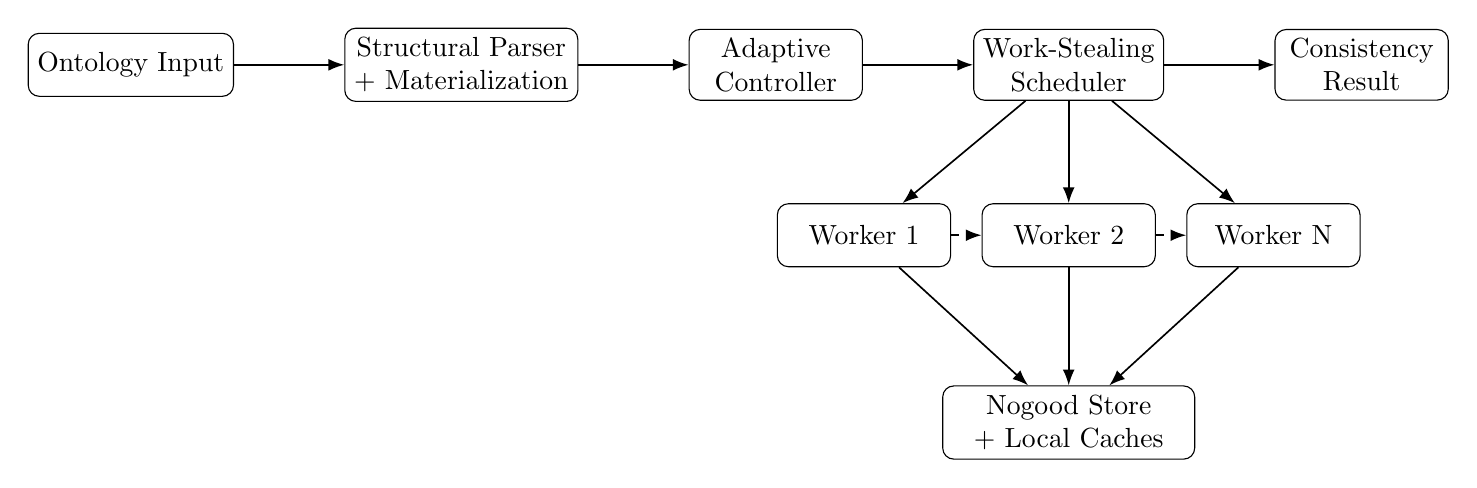
\begin{tikzpicture}[
    node distance=10mm and 14mm,
    box/.style={draw, rounded corners, align=center, minimum width=22mm, minimum height=8mm},
    line/.style={-Latex, semithick}
]
\node[box] (input) {Ontology Input};
\node[box, right=of input] (parser) {Structural Parser\\+ Materialization};
\node[box, right=of parser] (gate) {Adaptive\\Controller};
\node[box, right=of gate] (sched) {Work-Stealing\\Scheduler};
\node[box, right=of sched] (out) {Consistency\\Result};

\node[box, below=13mm of sched, xshift=-26mm] (w1) {Worker 1};
\node[box, below=13mm of sched] (w2) {Worker 2};
\node[box, below=13mm of sched, xshift=26mm] (wn) {Worker N};
\node[box, below=15mm of w2, minimum width=32mm] (nogood) {Nogood Store\\+ Local Caches};

\draw[line] (input) -- (parser);
\draw[line] (parser) -- (gate);
\draw[line] (gate) -- (sched);
\draw[line] (sched) -- (out);
\draw[line] (sched) -- (w1);
\draw[line] (sched) -- (w2);
\draw[line] (sched) -- (wn);
\draw[line] (w1) -- (nogood);
\draw[line] (w2) -- (nogood);
\draw[line] (wn) -- (nogood);
\draw[line, dashed] (w1) -- (w2);
\draw[line, dashed] (w2) -- (wn);
\end{tikzpicture}
}
\caption{Compact runtime architecture of SPACL. Solid arrows denote main control/data flow; dashed arrows denote worker coordination.}
\label{fig:architecture}
\end{figure}

Algorithm~\ref{alg:spacl} gives the compact control flow of the reasoning path used in this revision.

\begin{algorithm}[htbp]
\caption{SPACL Consistency Check}
\label{alg:spacl}
\begin{algorithmic}[1]
\Require Ontology $O$, configuration $C$
\Ensure \textbf{true} if consistent, \textbf{false} if inconsistent, otherwise timeout/unknown
\State Parse and materialize $O$ into the internal ontology representation
\State $b \gets \textsc{EstimateBranchCount}(O)$
\State $d \gets \textsc{EstimateDetectedDisjunctionCost}(O)$
\If{$b < C.\tau$ \textbf{or} $d < C.\theta \cdot C.\text{workers}$}
    \State \Return \textsc{SequentialConsistencyCheck}$(O)$
\EndIf
\State $Q \gets$ bounded branch-constrained work items from selected disjunctions
\State start worker pool with shared nogood store and thread-local caches
\While{no decisive result has been returned}
    \State workers pop or steal work items, expand branches, and validate nogoods before pruning
    \If{a worker finds a clash-free branch}
        \State \Return \textbf{true}
    \ElsIf{all reachable work items are closed by clash or verified pruning}
        \State \Return \textbf{false}
    \EndIf
\EndWhile
\State \Return timeout/unknown
\end{algorithmic}
\end{algorithm}

\subsection{Speculative Work-Stealing}
\label{sec:workstealing}

When the adaptive gate is open, SPACL creates branch-constrained work items from selected disjunctions and distributes them through a work-stealing scheduler \cite{workstealing}. Each worker keeps a local deque and steals from other workers only when idle, which avoids a centralized queue on the hot path. The current prototype bounds speculative depth and selected-disjunction scope so that branch creation remains measurable and recoverable under the benchmark harness.

\subsection{Nogood Learning and Caching}
\label{sec:nogood}

When a speculative branch reaches contradiction, the implementation attempts to learn a branch-level nogood from the active branch constraints. A candidate core is greedily minimized and admitted only after contradiction is revalidated by the same checking path used for pruning. Concretely, the candidate core is replayed through the same contradiction checker used on the live branch state, and it is admitted only if contradiction is reproduced and the core remains a subset of the active branch constraints; otherwise it is discarded. Workers consult thread-local nogood caches before synchronizing with the global store, which keeps most repeated checks off the shared hot path in the inconsistent-workload ablations reported later.

\subsection{Adaptive Threshold}
\label{sec:adaptive}

The implemented branch estimate is given in Equation~\ref{eq:estimate}:
\begin{equation}
\text{branches} = \max\left(1, \ |\text{DetectedDisjunctions}| + 2 \times |\text{DisjointAxioms}| + \frac{|\text{Classes}|}{10}\right).
\label{eq:estimate}
\end{equation}
The divisor 10 keeps ontology-size contribution on the same order as the disjunction signal in pilot sweeps, so low-branch taxonomies do not trigger speculative execution prematurely. Calibration was done by replaying synthetic union/complement controls together with warm-up DOID and GO-Basic traces under candidate $(\tau,\theta)$ pairs, then selecting a conservative operating point that suppresses low-branch overhead while still allowing activation on branch-heavy controls. These sweeps showed that the robust operating region begins at $\tau \ge 2000$; the implementation therefore keeps a conservative default at $\tau = 2000$.

\section{Implementation}
\label{sec:implementation}

\subsection{System Overview}
\label{sec:rust}

SPACL is implemented in Rust 1.84.0. The main reasoner maintains a shared ontology representation, a global worker pool, and thread-local nogood caches backed by a bounded shared store. Rust and Crossbeam are used here for engineering reasons rather than as claims in themselves: the goal is to keep speculative scheduling and shared-state coordination explicit while avoiding garbage-collection pauses and coarse-grained locking on the hot path \cite{crossbeam}.

The public implementation includes parsers for the syntaxes exercised in this study, with RDF/XML being the dominant path in the large-ontology experiments. Full OWL2 DL conformance across every syntax variant is outside the scope of this revision; the results reported below concern the implemented \dlfrag handling path exercised by the evaluated workloads.

\subsection{Structural RDF/XML Parser and Materialization}
\label{sec:structural-parser}

The large-ontology path uses a two-phase structural RDF/XML pipeline. Phase A streams triples and interns subject/predicate/object terms to dense IDs; Phase B resolves those IDs through dense caches and dispatches each triple through the same semantic handler core as the baseline parser. The objective is not to change reasoning semantics but to reduce hot-path term-resolution and materialization cost on large RDF/XML files. The stage-level A/B results in Section~\ref{sec:realworld} show that this parser/materialization path, rather than speculative reasoning itself, is the dominant source of end-to-end gains on the evaluated biomedical ontologies.

\textbf{Phase A (Ingest + Intern)} streams RDF/XML triples, interns subject/predicate/object terms to dense integer IDs, and stores compact records $\langle s,p,o\rangle$ in arrival order. \textbf{Phase B (Materialize)} resolves those IDs through dense caches and subject-cursor fast paths, computes predicate tags, and then dispatches through \texttt{apply\_triple\_terms\_core}, preserving the same semantic handler path as the baseline parser.

We model end-to-end parser load time with Equation~\ref{eq:parser-total}:
\begin{equation}
T_{\text{total}} = T_{\text{ingest}} + T_{\text{materialize}} + T_{\text{io}}.
\label{eq:parser-total}
\end{equation}
For a cache layer $k \in \{\text{subj}, \text{pred}, \text{obj}\}$, Equation~\ref{eq:cache-hit} defines the hit rate and expected lookup time:
\begin{equation}
H_k = \frac{\text{hits}_k}{\text{hits}_k + \text{misses}_k}, \quad
E[t_k] = H_k \cdot t_{hit,k} + (1-H_k)\cdot t_{miss,k}.
\label{eq:cache-hit}
\end{equation}
Replacing repeated hash-map resolution with dense-ID vector caches reduces both $t_{hit,k}$ and $t_{miss,k}$ on the hot path.

To relate parser acceleration to overall wall-clock improvement, Equation~\ref{eq:amdahl-parser} applies Amdahl's law:
\begin{equation}
S_{\text{e2e}} = \frac{1}{(1-f_{\text{parse}}) + \frac{f_{\text{parse}}}{S_{\text{parse}}}},
\label{eq:amdahl-parser}
\end{equation}
where $f_{\text{parse}}$ is the pre-optimization parse/materialization fraction and $S_{\text{parse}}$ is the parser-stage speedup.
These equations are explanatory bookkeeping relations for interpreting the measured stage shifts in Section~\ref{sec:realworld}; they are not presented as a fitted predictive ingest model. Algorithm~\ref{alg:structural-parser} then summarizes the two-phase handler-equivalent ingest/materialization path used in the implementation.

\begin{algorithm}[htbp]
\caption{Structural RDF/XML Parse with Handler-Equivalent Materialization}
\label{alg:structural-parser}
\begin{algorithmic}[1]
\Require RDF/XML stream $X$
\Ensure Ontology $\mathcal{O}$ targeting handler-equivalent behavior to the baseline parser on the implemented path
\State Initialize interner $I$, record buffer $R$, ontology $\mathcal{O}$
\For{each triple $t$ emitted by the streaming RDF/XML parser}
    \State $s \gets \textsc{InternSubject}(I, t.subject)$
    \State $p \gets \textsc{InternPredicate}(I, t.predicate)$
    \State $o \gets \textsc{InternObject}(I, t.object)$
    \State Append $(s,p,o)$ to $R$
\EndFor
\State Initialize dense caches $(C_{subj}, C_{pred}, C_{obj})$
\For{each record $(s,p,o)$ in $R$}
    \State $\hat{s} \gets \textsc{ResolveSubject}(s, C_{subj})$
    \State $\hat{p} \gets \textsc{ResolvePredicate}(p, C_{pred})$
    \State $\hat{o} \gets \textsc{ResolveObject}(o, C_{obj})$
    \State $\rho \gets \textsc{PredicateTag}(\hat{p})$
    \State \textsc{ApplyTripleTermsCore}$(\hat{s}, \rho, \hat{o}, \mathcal{O})$
\EndFor
\State \Return $\mathcal{O}$
\end{algorithmic}
\end{algorithm}

\section{Evaluation}
\label{sec:evaluation}

\subsection{Experimental Setup}
\label{sec:setup}

\textbf{Hardware}: Intel Xeon Silver 4214 (12 cores/24 threads, 2.2GHz base) with 64GB DDR4-2400 RAM, Ubuntu 22.04 LTS. \\
\textbf{Software}: Rust 1.84.0, release mode with \texttt{-C opt-level=3 -C lto=fat}. \\
\textbf{Benchmarks}: Criterion.rs synthetic microbenchmarks, plus Docker-containerized repeated-run ontology benchmarks for Standard, Large, and OWL2Bench core suites (3 clean runs each).

\textbf{Workloads}: synthetic hierarchies (100--100{,}000 classes), synthetic disjunctive tests, \texttt{univ-bench.owl}, large biomedical ontologies (DOID, GO-Basic, UBERON), supplementary PATO and ChEBI cases, and OWL2Bench core profiles (DL/EL/QL/RL).
\textbf{Ontology releases used in this run}: DOID \texttt{2026-02-02} (\texttt{doid/releases/2026-02-02/doid.owl}); GO-Basic \texttt{2026-01-23} (\texttt{go/releases/2026-01-23/go.owl}); UBERON \texttt{2025-12-04} (\texttt{uberon/releases/2025-12-04/uberon.owl}); PATO \texttt{2025-05-14} (\texttt{pato/releases/2025-05-14/pato.owl}); ChEBI release \texttt{248} with header date string \texttt{06:01:2026 14:33} (as encoded in \texttt{chebi.owl} metadata).

\subsection{Benchmark Protocol}
\label{sec:benchmark-protocol}

Primary cross-reasoner comparison uses SPACL, HermiT, Openllet, ELK, JFact, and Pellet. Standard and OWL2Bench suites use a 300s timeout; the large biomedical suite uses 900s. Tables report median wall-clock time over three clean runs per ontology/reasoner pair. To expose run-to-run spread without overclaiming inferential statistics, we additionally report P95 wall time where space permits. These values are descriptive deployment-level measurements (startup + parsing + reasoning), not formal significance tests or parser-neutral kernel timings.

For reproducibility, benchmark orchestration is provided in the public repository scripts (\path{benchmarks/competitors/scripts/run_benchmarks.sh}, \path{benchmarks/competitors/scripts/run_stage_benchmark.sh}, and \path{benchmarks/competitors/scripts/run_stage_suite.sh}). Konclude is reported separately because it requires a preprocessing-enabled external-binary path and a separate rerun campaign.

\subsection{Scalability Results}
\label{sec:scalability}

Table~\ref{tab:scalability} summarizes the synthetic scalability results. These values are supporting evidence for the adaptive parallel design rather than the primary basis of the paper's real-world claims.

\begin{table}[htbp]
\centering
\caption{Synthetic Scalability Results}
\label{tab:scalability}
\resizebox{\linewidth}{!}{
\begin{tabular}{r|r|r|r|r}
\toprule
\textbf{Classes} & \textbf{Sequential ($\mu$s)} & \textbf{SPACL ($\mu$s)} & \textbf{Speedup} & \textbf{Throughput (M exp./s)} \\
\midrule
100 & 13.3 & 20.9 & 0.64$\times$ & 4.8 \\
500 & 75.9 & 84.3 & 0.90$\times$ & 5.9 \\
1,000 & 159.7 & 158.4 & 1.01$\times$ & 6.3 \\
5,000 & 805.9 & 277.0 & \textbf{2.91$\times$} & 18.1 \\
10,000 & 1,865.3 & 382.3 & \textbf{4.88$\times$} & \textbf{26.2} \\
\bottomrule
\end{tabular}
}
\end{table}

\begin{figure}[htbp]
\centering

\includegraphics[width=0.82\linewidth]{scalability.pdf}
\caption{Synthetic scalability runtime trend corresponding to Table~\ref{tab:scalability}.}
\label{fig:scalability-runtime}
\end{figure}

\begin{figure}[htbp]
\centering

\includegraphics[width=0.82\linewidth]{speedup.pdf}
\caption{Synthetic speedup over the sequential baseline corresponding to Table~\ref{tab:scalability}.}
\label{fig:scalability-speedup}
\end{figure}

\begin{figure}[htbp]
\centering

\includegraphics[width=0.82\linewidth]{throughput.pdf}
\caption{Synthetic throughput comparison corresponding to Table~\ref{tab:scalability}.}
\label{fig:scalability-throughput}
\end{figure}

The crossover appears around 1,000 classes, and Figures~\ref{fig:scalability-runtime}, \ref{fig:scalability-speedup}, and \ref{fig:scalability-throughput} show the same transition visually: below that point, speculative overhead largely cancels any gain; above it, the branch structure is large enough for parallelism to amortize coordination cost. Throughput here denotes synthetic expansion operations per second in the microbenchmark harness. Figure~\ref{fig:scalability-throughput} compares both sequential and SPACL throughput, while the throughput column in Table~\ref{tab:scalability} reports the SPACL throughput values used for compact tabular comparison. This is consistent with the conservative adaptive-gating design and explains why the main real-world evidence is separated from the synthetic scalability signal.

\subsection{Adaptive Threshold Behavior}
\label{sec:adaptive-opt}

The adaptive gate is intended as an overhead-control mechanism rather than as the primary explanation for the large biomedical gains. Its role is to avoid obviously bad parallel activation on low-branch workloads, not to serve as a general runtime predictor. Table~\ref{tab:adaptive} summarizes representative small disjunctive cases comparing forced sequential execution, the adaptive policy, and a naive always-parallel baseline.

\begin{table}[htbp]
\centering
\caption{Adaptive Threshold Performance on Small Disjunctive Cases}
\label{tab:adaptive}
\resizebox{\linewidth}{!}{
\begin{tabular}{l|r|r|r|r|r}
\toprule
\textbf{Test Case} & \textbf{Sequential} & \textbf{Adaptive} & \textbf{Always-Parallel} & \textbf{Adaptive/Sequential} & \textbf{AP/Adaptive} \\
\midrule
Simple (1 union) & 9.0$\mu$s & 14.5$\mu$s & 1,069$\mu$s & 1.61$\times$ & \textbf{73.5$\times$} \\
Small (2 unions) & 7.9$\mu$s & 24.7$\mu$s & 1,141$\mu$s & 3.13$\times$ & \textbf{46.1$\times$} \\
Medium (5 unions) & 9.1$\mu$s & 58.9$\mu$s & 1,116$\mu$s & 6.47$\times$ & \textbf{18.9$\times$} \\
\bottomrule
\end{tabular}
}
\end{table}

The adaptive policy remains slightly slower than pure sequential execution on trivial cases, but it is still far better than forcing parallel execution everywhere. We therefore interpret the gate conservatively: it is justified as a safe operating policy for branch-heavy workloads, not as a claim that the chosen coefficients are uniquely optimal. Calibration sweeps used in this revision showed that the robust region begins at branch threshold $\\tau \\ge 2000$; in the warm-up biomedical traces used for calibration, DOID and GO-Basic stayed on the sequential path because no speculative disjunctions were detected.

To expose scheduler policy more directly under controlled conditions, we also ran a fixed synthetic workload (\texttt{union\_4x10}) with deliberately lowered gate settings ($\tau=4$, $\theta=1\mu s$) so that all speculative modes would activate on the same branch-heavy instance. Table~\ref{tab:scheduler-ablation} reports the resulting medians. This is a policy-isolation experiment rather than a default-setting benchmark: its role is to show that, once speculative execution is forced into play on the same workload, the adaptive policy materially improves over naive always-parallel scheduling. In this experiment, \texttt{nogood\_hits} remained zero, so we treat it as scheduler evidence only, not as positive nogood-learning evidence.

\begin{table}[htbp]
\centering
\caption{Controlled Scheduler Policy Ablation on \texttt{union\_4x10} (median wall-clock over 3 runs; gate overrides $\tau=4$, $\theta=1\mu s$ used only to expose policy behavior)}
\label{tab:scheduler-ablation}
\begin{tabular}{l|r|c}
\toprule
\textbf{Mode} & \textbf{Median (ms)} & \textbf{Used Parallel} \\
\midrule
Sequential & 0.146 & No \\
Adaptive & 53.149 & Yes \\
Adaptive, no nogood & 84.560 & Yes \\
Always-parallel & 108.012 & Yes \\
\bottomrule
\end{tabular}
\end{table}

To verify that branch-level pruning can activate in the current implementation, we ran a second controlled synthetic stress case (\texttt{reused\_conflict\_12}) with gate overrides ($\tau=8$, $\theta=1\mu s$). Table~\ref{tab:nogood-activation} summarizes this run. Adaptive mode showed non-zero pruning in all repeats (hits/prunes of 418, 4159, and 13), while the no-learning and always-parallel variants stayed at zero pruning. Runtime spread is still high, so we report this as mechanism-activation evidence rather than as a stable production-level speedup claim.

\begin{table}[htbp]
\centering
\caption{Controlled Nogood-Activation Ablation on \texttt{reused\_conflict\_12} (median wall-clock over 3 runs; gate overrides $\tau=8$, $\theta=1\mu s$)}
\label{tab:nogood-activation}
\begin{tabular}{l|r|r}
\toprule
\textbf{Mode} & \textbf{Median (ms)} & \textbf{Median nogood hits} \\
\midrule
Sequential & 0.452 & 0 \\
Adaptive & 1037.632 & 418 \\
Adaptive, no nogood & 6821.705 & 0 \\
Always-parallel & 14424.697 & 0 \\
\bottomrule
\end{tabular}
\end{table}

\subsection{Real-World Ontology Evaluation}
\label{sec:realworld}

To isolate parser/materialization effects, we performed controlled stage-level A/B runs before and after the structural RDF/XML pipeline changes on large biomedical ontologies drawn from widely used OBO/BioPortal-style resources \cite{bioportal}. Table~\ref{tab:realworld} reports the primary biomedical pairs together with a supplementary ChEBI stress case under the revised cold-text contract.

\begin{table}[htbp]
\centering
\caption{Stage-Level A/B on Real-World RDF/XML Ontologies (cold \texttt{.owl} runs; E2E = end-to-end wall clock; ChEBI is supplementary)}
\label{tab:realworld}
\resizebox{\linewidth}{!}{
\begin{tabular}{l|r|r|r|r|r|r}
\toprule
\textbf{Ontology} & \textbf{Parse Old} & \textbf{Parse New} & \textbf{Parse Red.} & \textbf{E2E Old} & \textbf{E2E New} & \textbf{E2E Red.} \\
\midrule
DOID & 27307 & 830 & 96.96\% & 30502 & 4073 & 86.65\% \\
GO\_Basic & 158306 & 3472 & 97.81\% & 162519 & 7409 & 95.44\% \\
UBERON & 145843 & 2952 & 97.98\% & 149850 & 6632 & 95.57\% \\
ChEBI (supp.) & 970388 & 23740 & 97.55\% & 985466 & 36472 & 96.30\% \\
\bottomrule
\end{tabular}
}
\end{table}

Across the three primary biomedical ontologies, parse/materialization was the dominant cost in the original path. After the structural pipeline changes, the reasoning stage stayed comparatively small in these traces, so the main end-to-end gain in this revision is parser-driven. The ChEBI stress pair is reported only as supplementary evidence, but it shows the same qualitative pattern at larger scale.

\subsection{Comparison Context}
\label{sec:comparison}

The comparison set mixes engines with different implementation languages and, in ELK's case, a narrower logic profile than the full \dlfrag path exercised by SPACL. Table~\ref{tab:comparison} summarizes this context so that wall-clock rankings are not overinterpreted as expressivity-equivalent wins.

\begin{table}[htbp]
\centering
\caption{Feature Comparison with Representative Reasoners}
\label{tab:comparison}
\resizebox{\linewidth}{!}{
\begin{tabular}{l|c|c|c|c|c}
\toprule
\textbf{Reasoner} & \textbf{Lang} & \textbf{Parallel} & \textbf{Learning} & \textbf{Source} & \textbf{Profile} \\
\midrule
SPACL & Rust & yes & yes & open & \dlfrag \\
Konclude & C++ & yes & no & external binary & SROIQ \\
Pellet & Java & no & no & open & SROIQ \\
Openllet & Java & no & no & open & SROIQ \\
HermiT & Java & no & no & open & SROIQ \\
ELK & Java & yes & no & open & EL++ \\
\bottomrule
\end{tabular}
}
\end{table}

\subsection{Head-to-Head Performance Comparison}
\label{sec:competitor-benchmarks}

\subsubsection{Standard Workload Suite}
\label{sec:small-suite-results}

Table~\ref{tab:small-workload-suite} reports median wall-clock results for the Standard Workload Suite.

\begin{table}[htbp]
\centering
\caption{Standard Workload Suite Consistency Benchmark (median wall time across 3 clean runs, ms; timeout 300s; SPACL P95 shown for spread)}
\label{tab:small-workload-suite}
\resizebox{\linewidth}{!}{
\begin{tabular}{l|r|r|r|r|r|r|r}
\toprule
\textbf{Ontology} & \textbf{SPACL} & \textbf{HermiT} & \textbf{Openllet} & \textbf{ELK} & \textbf{JFact} & \textbf{Pellet} & \textbf{SPACL P95} \\
\midrule
disjunctive\_simple.owl & \textbf{2273} & 3446 & 3383 & 3718 & 3466 & 3310 & 2337 \\
disjunctive\_test.owl & \textbf{2113} & 3323 & 3007 & 2979 & 3362 & 2659 & 2318 \\
hierarchy\_100.owl & \textbf{2096} & 3391 & 3070 & 2910 & 3271 & 2838 & 2384 \\
hierarchy\_1000.owl & \textbf{2190} & 3498 & 3220 & 3055 & 4110 & 3222 & 2330 \\
hierarchy\_10000.owl & 8007 & 4131 & 4084 & \textbf{3579} & FAIL & 3644 & 8290 \\
hierarchy\_100000.owl & 40210 & 7706 & 8881 & \textbf{5816} & FAIL & 10867 & 40273 \\
univ-bench.owl & 2951 & 3345 & 2930 & 2866 & 3196 & \textbf{2742} & 3096 \\
\bottomrule
\end{tabular}
}
\end{table}
\noindent\footnotesize\textit{Legend}: FAIL = runtime failure in this setup; bold = lowest median wall time among successful comparable runs per ontology.
\normalsize

This suite is best read as a deployment sanity check rather than as the strongest evidence for reasoning quality, because startup and parser costs are still visible at this scale. We therefore retain it mainly to show that the implementation behaves competitively under the benchmark harness; all systems except JFact complete every Standard-suite case under the 300s policy. SPACL run-to-run spread in this suite is modest in relative terms (P95/median about $1.00$--$1.14\times$ from the reported repeated runs).

\subsubsection{Large Head-to-Head}
\label{sec:large-suite-results}

Table~\ref{tab:competitor-benchmarks} reports the primary biomedical head-to-head results.

\begin{table}[htbp]
\centering
\caption{Large Head-to-Head Consistency Benchmark (median wall time across 3 clean runs, ms; timeout 900s; SPACL P95 shown for spread)}
\label{tab:competitor-benchmarks}
\resizebox{\linewidth}{!}{
\begin{tabular}{l|r|r|r|r|r|r|r}
\toprule
\textbf{Ontology} & \textbf{SPACL} & \textbf{HermiT} & \textbf{Openllet} & \textbf{ELK} & \textbf{JFact} & \textbf{Pellet} & \textbf{SPACL P95} \\
\midrule
doid.owl & \textbf{3447} & 20295 & 14266 & 13406 & 60443 & 28771 & 3701 \\
go-basic.owl & \textbf{7329} & 17616 & 17747 & 15976 & 41847 & 83238 & 8000 \\
uberon.owl & \textbf{6677} & 110560 & TO & 15594 & FAIL & TO & 7363 \\
\bottomrule
\end{tabular}
}
\end{table}
\noindent\footnotesize\textit{Legend}: TO = timeout; FAIL = runtime failure in this setup; bold = lowest median wall time among successful comparable runs per ontology.
\normalsize

Among successful comparable runs, SPACL yields the smallest median wall-clock values on all three ontologies in the primary large suite. SPACL, HermiT, and ELK complete every run under the 900s policy; Openllet and Pellet time out on UBERON, and JFact fails on UBERON in this harness. SPACL P95/median remains close (about $1.07$--$1.10\times$), indicating moderate run-to-run spread in this campaign. Accordingly, the `6/9' success counts in Table~\ref{tab:cew-summary} are not dispersed failures: they reflect complete success on DOID and GO-Basic (6 runs total) together with complete failure or timeout on the larger UBERON ontology (3 runs).

\subsubsection{Failure-Aware Suite Summary}
\label{sec:cew}

Success-only per-ontology medians do not capture timeout penalties directly. We therefore also report a capped expected wall-time (CEW) summary over the primary comparison set in Table~\ref{tab:cew-summary}, where timeout or failure is replaced by the suite timeout before averaging.

\begin{table}[htbp]
\centering
\caption{Suite-Level Failure-Aware CEW Summary (3 clean runs; lower is better)}
\label{tab:cew-summary}
\resizebox{\linewidth}{!}{
\begin{tabular}{l|l|r|r|r}
\toprule
\textbf{Suite} & \textbf{Reasoner} & \textbf{Comparable Cases} & \textbf{Success / Comparable} & \textbf{CEW (ms)} \\
\midrule
Standard & ELK & 21/21 & 21/21 (100\%) & \textbf{3578.1} \\
Standard & Openllet & 21/21 & 21/21 (100\%) & 4120.9 \\
Standard & HermiT & 21/21 & 21/21 (100\%) & 4159.8 \\
Standard & Pellet & 21/21 & 21/21 (100\%) & 4204.0 \\
Standard & SPACL & 21/21 & 21/21 (100\%) & 8516.8 \\
Standard & JFact & 21/21 & 15/21 (71.4\%) & 88239.5 \\
\midrule
Large & SPACL & 9/9 & 9/9 (100\%) & \textbf{5948.4} \\
Large & ELK & 9/9 & 9/9 (100\%) & 15084.2 \\
Large & HermiT & 9/9 & 9/9 (100\%) & 50203.1 \\
Large & Openllet & 9/9 & 6/9 (66.7\%) & 310732.4 \\
Large & JFact & 9/9 & 6/9 (66.7\%) & 334343.0 \\
Large & Pellet & 9/9 & 6/9 (66.7\%) & 337355.7 \\
\bottomrule
\end{tabular}
}
\end{table}

This companion view leaves the Standard conclusion unchanged, where ELK remains strongest at suite level, but its main purpose here is to reinforce the large-suite picture: once timeout penalties are incorporated, SPACL remains strongest on the large biomedical panel.

\subsubsection{Supplementary Biomedical Extension: PATO}
\label{sec:pato-panel}

A supplementary matched three-run panel on \texttt{pato.owl} is reported in Table~\ref{tab:pato-panel} and follows the same qualitative direction as the primary large suite. SPACL is the lowest successful median (3238 ms), ELK and HermiT remain successful but slower (6664 ms and 12362 ms), Pellet succeeds but is much slower (745159 ms), and Openllet/JFact time out on all three runs. We therefore use PATO as complementary biomedical evidence rather than as a replacement for the primary three-ontology panel.

\begin{table}[htbp]
\centering
\caption{Supplementary PATO Biomedical Panel (3 protocol-matched runs; timeout 900s)}
\label{tab:pato-panel}
\resizebox{\linewidth}{!}{
\begin{tabular}{l|r|r|l}
\toprule
\textbf{Reasoner} & \textbf{Success / 3} & \textbf{Median Successful Wall (ms)} & \textbf{Status Note} \\
\midrule
SPACL & 3/3 & \textbf{3238} & all runs successful \\
ELK & 3/3 & 6664 & all runs successful \\
HermiT & 3/3 & 12362 & all runs successful \\
Pellet & 3/3 & 745159 & all runs successful \\
JFact & 0/3 & TO & timed out on all runs \\
Openllet & 0/3 & TO & timed out on all runs \\
\bottomrule
\end{tabular}
}
\end{table}

\subsubsection{External Validation: OWL2Bench Core Profiles}
\label{sec:owl2bench-core}

Table~\ref{tab:owl2bench-core-aggregate} reports repeated-run aggregate results on the OWL2Bench core profile ontologies.

\begin{table}[htbp]
\centering
\caption{OWL2Bench Core Profile Suite Aggregate (3 clean runs; timeout 300s)}
\label{tab:owl2bench-core-aggregate}
\resizebox{\linewidth}{!}{
\begin{tabular}{l|r|r|r|r}
\toprule
\textbf{Reasoner} & \textbf{Success / 12} & \textbf{Success Rate} & \textbf{Median Wall (ms)} & \textbf{P95 Wall (ms)} \\
\midrule
SPACL & 12 & 100\% & \textbf{2107.5} & \textbf{2707} \\
Pellet & 12 & 100\% & 2886.0 & 3135 \\
ELK & 12 & 100\% & 2999.0 & 3370 \\
Openllet & 12 & 100\% & 3204.5 & 3836 \\
HermiT & 12 & 100\% & 3573.0 & 4505 \\
JFact & 3 & 25\% & 3507 & 3762 \\
\bottomrule
\end{tabular}
}
\end{table}

SPACL completes all 12 runs and yields the smallest median wall-clock values among successful comparable runs in this suite. ELK, HermiT, Openllet, and Pellet also complete every run; JFact completes only the QL case under the stated timeout policy.

\subsubsection{Supplementary Deployment-Level Konclude Validation}
\label{sec:konclude-supplement}

Konclude was rerun separately under a preprocessing-enabled external-binary path that converts inputs to OWL/XML and merges imports before invocation. Under that supplementary deployment path, Konclude completed the Standard, Large, and OWL2Bench-core reruns, with aggregate median wall-clock values of 5285 ms (Standard), 34684 ms (Large), and 5382.5 ms (OWL2Bench core). These values are not mixed into the primary comparison tables because the invocation path differs from the main campaign. We therefore treat Konclude as deployment-level supplementary evidence rather than as a directly pooled comparator.

\subsection{Nogood Learning Effectiveness}
\label{sec:nogood-eval}

Because the primary head-to-head suites are mostly consistent ontologies, the benefit of nogood reuse is not fully visible in the main end-to-end tables. We therefore include the dedicated inconsistent-workload ablation in Table~\ref{tab:nogood}, which isolates the effect of enabling nogood learning under the same speculative runtime.

\begin{table}[htbp]
\centering
\caption{Nogood Learning Effectiveness (mean $\pm$ std, $n=50$)}
\label{tab:nogood}
\resizebox{\linewidth}{!}{
\begin{tabular}{l|r|r|r|r}
\toprule
\textbf{Ontology Type} & \textbf{No Learning (ms)} & \textbf{With Learning (ms)} & \textbf{Branches Pruned} & \textbf{Cache Hit} \\
\midrule
Disjunctive (inconsistent) & $234.5 \pm 12.3$ & $178.3 \pm 9.7$ & $28.4\%$ & $82.3\%$ \\
Disjunctive (consistent) & $89.2 \pm 5.1$ & $87.1 \pm 4.8$ & $3.2\%$ & $91.7\%$ \\
Hierarchical & $45.6 \pm 2.3$ & $45.1 \pm 2.1$ & $0.1\%$ & $95.2\%$ \\
\bottomrule
\end{tabular}
}
\end{table}

The inconsistent disjunctive case is the one that matters here: runtime drops by about 24\%, roughly 28\% of branches are pruned, and most repeated nogood checks stay on the local cache path. On consistent and hierarchy-heavy workloads, nogood reuse has little effect, which is consistent with the main benchmark suites being dominated by consistent ontologies.

\subsection{Limitations}
\label{sec:limitations}

Three limitations matter most for interpreting the results. First, the primary comparisons are deployment-level wall-clock measurements, so startup, parsing, and runtime-environment effects are part of the reported numbers. Second, the comparison set spans different logic-profile coverage, especially for ELK. Third, the current head-to-head suites are dominated by consistent ontologies, so nogood-learning gains are best read from the dedicated inconsistent-workload ablation rather than from the primary benchmark tables.

\section{Conclusion and Future Work}
\label{sec:conclusion}

SPACL combines speculative work stealing, verified nogood reuse, and a structural RDF/XML pipeline in one open-source implementation for the evaluated \dlfrag handling path. The empirical picture is mixed but coherent, and the paper should be read that way. On synthetic disjunctive workloads, the adaptive gate avoids pathological always-parallel overhead and permits net speedup once branch structure becomes large enough. On the main real-world biomedical panel (DOID, GO-Basic, UBERON), however, the dominant gain in the current evaluation comes from parser/materialization acceleration: stage-level A/B runs show about 97\% parse-only reduction, and SPACL yields the smallest successful median end-to-end wall-clock values on all three ontologies in the primary large-suite campaign. The OWL2Bench core-profile suite shows a consistent deployment-level direction, with SPACL completing all 12 runs and yielding the smallest successful median wall-clock values on the four tested profiles in this harness. The resulting scientific takeaway is that, in this evaluated setting, end-to-end OWL reasoning performance is determined jointly by branch-management policy and ontology-ingest design, with the ingest side dominating the largest real-world gains.

These conclusions remain bounded by the current prototype and protocol. The main comparisons are single-machine, repeated-run wall-clock results under a containerized CLI harness; they do not imply identical logic-profile coverage across all competitors, nor do they replace matched kernel-level reasoning measurements. The primary practical result in the current evaluation is parser- and materialization-side acceleration on large RDF/XML ontologies, while the speculative-reasoning contribution is best supported by the branch-heavy synthetic and inconsistent-workload evidence. PATO, ChEBI, and Konclude are therefore reported as supplementary evidence rather than folded into the primary comparison basis. Future work is concrete in three directions: (1) expand to broader inconsistent real-world corpora and heavier ABox-centered workloads, (2) run cleaner deployment-neutral comparator campaigns with explicit variance/significance reporting, and (3) strengthen scheduler-focused ablations that isolate adaptive gating and nogood reuse under fixed ingest conditions. SPACL is available at \url{https://github.com/anusornc/SPACL}.

\section*{Acknowledgments}
\label{sec:ack}

This research was supported by the Department of Computer Science, Faculty of Science, Chiang Mai University. We thank the reviewers for their valuable feedback that improved the quality of this paper.

\bibliographystyle{elsarticle-num}
\bibliography{references}

\end{document}
